\documentclass[10pt,twocolumn,letterpaper]{article}

% \usepackage{cvpr}
\usepackage{times}
\usepackage{epsfig}
\usepackage{graphicx}
\usepackage{amsmath}
\usepackage{amssymb}

% Include other packages here, before hyperref.

% If you comment hyperref and then uncomment it, you should delete
% egpaper.aux before re-running latex.  (Or just hit 'q' on the first latex
% run, let it finish, and you should be clear).
\usepackage[breaklinks=true,bookmarks=false]{hyperref}


\begin{document}


%%%%%%%%% TITLE
\title{Learning pixel objectness with Positive and Unlabelled examples}

\author{First Author\\
Institution1\\
Institution1 address\\
{\tt\small firstauthor@i1.org}
% For a paper whose authors are all at the same institution,
% omit the following lines up until the closing ``}''.
% Additional authors and addresses can be added with ``\and'',
% just like the second author.
% To save space, use either the email address or home page, not both
\and
Second Author\\
Institution2\\
First line of institution2 address\\
{\tt\small secondauthor@i2.org}
}

\maketitle
%\thispagestyle{empty}


%%%%%%%%% ABSTRACT
\begin{abstract}
   The ABSTRACT HERE
\end{abstract}

%%%%%%%%% BODY TEXT
\section{Bullet points}


\paragraph{Data for Semantic Segmatation}
\begin{itemize}
  \item Rich unlabeled data, but lack of annotations
  \item (Conventionally) The annotations need to be:
  \begin{itemize}
    \item \textbf{precise}: no false positive
    \item \textbf{complete}: no false negative
    \item \textbf{consistent}: no misclassification
  \end{itemize}

  % \item (Conventional) Workflow:
  % \begin{enumerate}
  %   \item Filter out the irrelavant images
  %   \item Annotate the relavant images
  %   \item Iterate for multiple times Step 1. and 2.
  % \end{enumerate}

  \item Annotations that
  \begin{itemize}
      \item contain \textbf{imprecise} annotations
      \item are \textbf{imcomplete}
      \item contain \textbf{misclassification}
  \end{itemize}

  % \item Motivation:
  % \begin{itemize}
  %   \item Correcting annotation errors take much more effort than annotating more data
  %   \item Annotation errors could be compensated with appropriate assumptions
  % \end{itemize}
\end{itemize}


\paragraph{Methods}
\begin{itemize}
  \item Incomplete annotations: Positive and Unlabelled learning
  \item Imprecise annotations: Learning ``objectness''
  \item Inconsistent classifications: ``Bootstrapping''(Entropy Regularization), Linear Noise model, Dropout Regularization
\end{itemize}


\section{Introduction}
\label{introduction}



%%%%%%%%%%%%%%%%%%%%%%%%%%%%%%%%%%%%%%%%%%%%%%%%%%%%%%%%%%%%%%%%%%%%%%
%%%%%%%% Figure 1
%%%%%%%%%%%%%%%%%%%%%%%%%%%%%%%%%%%%%%%%%%%%%%%%%%%%%%%%%%%%%%%%%%%%%%

\begin{figure}[t]
\begin{center}
% \fbox{\rule{0pt}{2in} \rule{0.9\linewidth}{0pt}}
   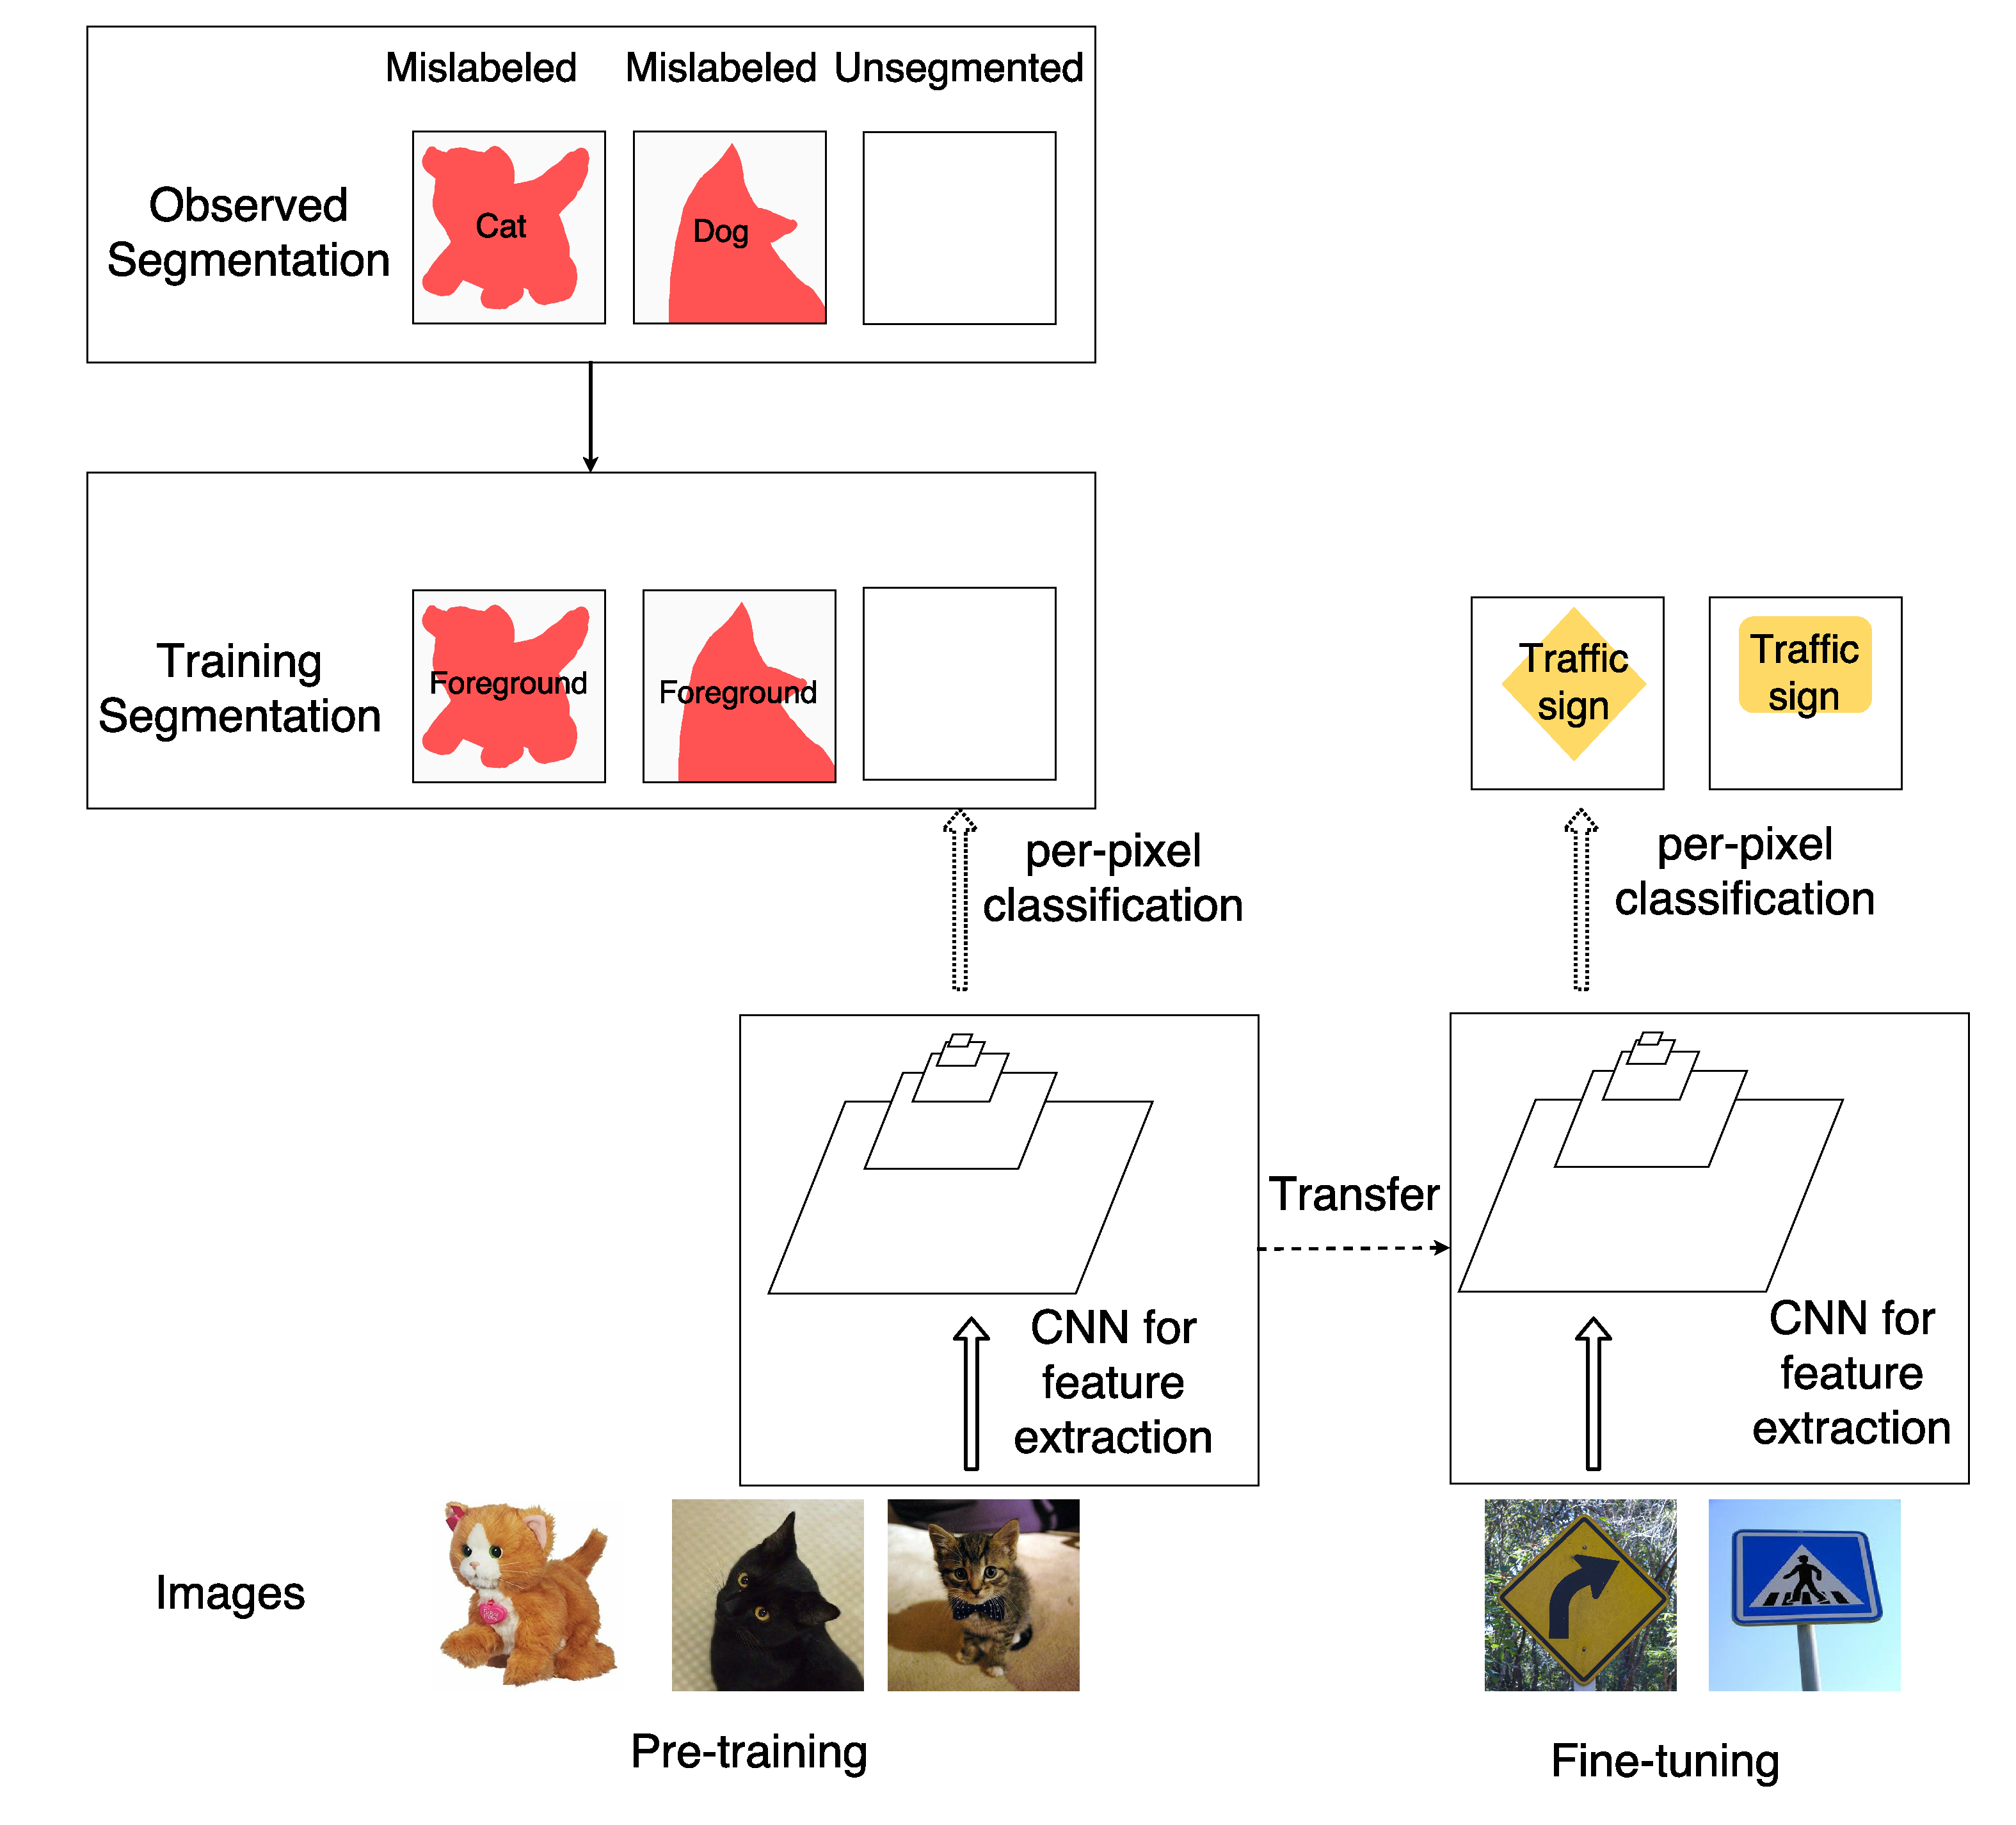
\includegraphics[width=1.0\linewidth]{img/figure1}
\end{center}
   \caption{
   Learning representations with segmentation datasets that potentially contains mislabeled objects and missing segmentation.
   We propose (1) to train with only segmentations instead of labeled segmentations, (2) to apply a sigmoid loss for the background class.
   The learned representations are then used as weights initialization and fine-tuned with a small set of true labels in the domain of interest.
   }
\label{fig:figure1}
\end{figure}


%%%%%%%%%%%%%%%%%%%%%%%%%%%%%%%%%%%%%%%%%%%%%%%%%%%%%%%%%%%%%%%%%%%%%%
%%%%%%%% TEXT Why transfer learning?
%%%%%%%%%%%%%%%%%%%%%%%%%%%%%%%%%%%%%%%%%%%%%%%%%%%%%%%%%%%%%%%%%%%%%%

% \noindent \textit{Why transfer learning? \\
% Segmentation model benefits from transfer learning.
% \begin{itemize}
%   \item Success of CNN benefits from large-scale data whereas segmentation datasets are small
%   \item Collecting segmentation in one domain on a large scale can be difficult.
%   \item One can transfer pre-trained CNN model to train with limited training samples access.
% \end{itemize}
% }

The often limited availability of training samples motivates most state-or-the-art deep learning based segmentation models \cite{long2015fully,chen2016deeplab,he2017mask} to transfer convolutional neural network (CNN) models \cite{krizhevsky2012imagenet,simonyan2014very,szegedy2015going,he2016deep} trained on a subset of images from ImageNet.
% The pre-trained models \cite{krizhevsky2012imagenet,simonyan2014very,szegedy2015going,he2016deep} are normally trained on an object recognition task, the ILSVRC \cite{russakovsky2015imagenet} challenge, using around 1.2 million labeled images.
% Compared to object recognition tasks, it is tougher to collect a dataset for semantic segmentation on a large scale.
The difficulty of obtaining manual segmentations is natural because it costs much more efforts for people to segment than to classify an image.
One of the largest segmentation datasets, Microsoft COCO2014 \cite{lin2014microsoft}, contains 123,287 images of 80 object categories.
As a comparison, a well-known successful task for convolutional neural networks, object recognition on the ILSRVC dataset\cite{russakovsky2015imagenet}, has around 1.2 million images for 1000 categories to train.
% the Pascal VOC2012 challenge \cite{everingham2015pascal} provides a segmentation dataset with only 9,993 segmented images for 20 object categories;
% The PASCAL-context Dataset \cite{mottaghi2014role} enriches the PASCAL VOC dataset by segmenting all 11,530 training images for 540 categories;
Transferring weights from the pre-trained ImageNet models can provide a segmentation performance boost in the limitation of lacking training samples, as reported in \cite{long2015fully} and adopted by \cite{chen2016deeplab,he2017mask}.
But the pre-trained ImageNet models are originally designed for object recognition problems, which can cause more problems than it solves.

%%%%%%%%%%%%%%%%%%%%%%%%%%%%%%%%%%%%%%%%%%%%%%%%%%%%%%%%%%%%%%%%%%%%%%
%%%%%%%% TEXT Why pre-training with segmentation?
%%%%%%%%%%%%%%%%%%%%%%%%%%%%%%%%%%%%%%%%%%%%%%%%%%%%%%%%%%%%%%%%%%%%%%

% \noindent \textit{Why pre-training with segmentation? \\
% ImageNet models have limitations.
% \begin{itemize}
%   \item Disimilarity in domain of interest for training images
%   \item Architecture limitation of ImageNet models. (3D ConvNet)
% \end{itemize}
% }

In practice, it can be challenging to employ representations from the ImageNet CNN models directly for segmentation.
Firstly, the object recognition models pursue features invariance to better capture semantics regardless the variations in objects.
The result translation invariant and resolution-reduced features reduce the localization accuracy which is not essential for object recognition but is critical for object segmentation. \cite{zheng2015conditional,chen2016deeplab}
Secondly, the ImageNet models were originally trained with natural images at relatively low resolution.
However, images to be segmented may (1) have a third dimension (3D images like CT scans and MRI scans), (2) contain extra channels (RGB-D images),  (3) be non-natural, such as aerial images and medical images.
These issues prevent transferring representations of the ImageNet models from improving segmentation performance significantly.
In this case, it can be beneficial to retrain the pre-trained ImageNet models with segmentation datasets for fine-grained cues about boundaries in the domain.

% \footnote{The KITTI Vision Benchmark Suite http://www.cvlibs.net/datasets/kitti/}

%%%%%%%% ? Deeplab https://arxiv.org/pdf/1606.00915.pdf
%%%%%%%% In particular we consider three challenges in the application of DCNNs to semantic image segmentation: (1) reduced feature resolution, (2) existence of objects at multiple scales, and (3) reduced localization accuracy due to DCNN invariance.
%%%%%%%% ? CRFasRNN http://www.robots.ox.ac.uk/~szheng/papers/CRFasRNN.pdf
%%%%%%%% Firstly, traditionalCNNs have convolutional filters with large receptivefields and hence produce coarse outputs when restructured to produce pixel-level labels [37]
%%%%%%%% Secondly, CNNs lack smoothness constraints that encourage label agreement between similar pixels, and spatial and appearance consistency of the labelling output


%%%%%%%%%%%%%%%%%%%%%%%%%%%%%%%%%%%%%%%%%%%%%%%%%%%%%%%%%%%%%%%%%%%%%%
%%%%%%%% TEXT Why labels are noisy?
%%%%%%%%%%%%%%%%%%%%%%%%%%%%%%%%%%%%%%%%%%%%%%%%%%%%%%%%%%%%%%%%%%%%%%

% \noindent
% \textit{Why labels are noisy?
% \begin{itemize}
%   \item Crowd-sourcing data is noisy by nature.
%   \item ``gold standard'' itself can be ambiguous.
%   \item There exists free available noisy segmentation datasets
% \end{itemize}
% }

The segmentation datasets for pre-training representations may contain label errors.
The use of the crowd-sourcing platform like Mechanical Turk is common nowadays to collect annotations on a large-scale.
It is natural for crowd-sourcing workers to make mistakes as a result of lack of expertise, inherent ambiguity of tasks or unconscious bias.
Enormous efforts are required, according to  \cite{lin2014microsoft,everingham2015pascal}, to ensure the correctness of segmentations.
%A slight decrease in the percentage of segmentation errors, such as from 1\% to 0\%, may require extraordinary extra efforts due to the difficulty of identifying errors.
% If not requiring ``gold standard'' segmentations for training, the efforts saved for correctness can be made to segment more images for a larger dataset.
%In some domains, for example, medical imaging, the ``gold standard'' itself can be ambiguous and cause disagreements among experts.
In addition, automated labels other than the manual ones may be freely available for particular tasks.
For example, segmentations of road and buildings for aerial images can be derived from digital maps, like OpenStreetMap, by aligning images to maps.
However, segmentations constructed in this way suffer from incompleteness as well as registration problems \cite{mnih2012learning}.
% Besides, Pl@ntNet\footnote{https://identify.plantnet-project.org/}, a crowdsourcing platform, provide millions of images of plants and corresponding labels which may or may not be correct.
Ideally, label errors in segmentations should not significantly affect the learned representations and its transferability to other datasets.

%%%%%%%%%%%%%%%%%%%%%%%%%%%%%%%%%%%%%%%%%%%%%%%%%%%%%%%%%%%%%%%%%%%%%%
%%%%%%%% TEXT What types of noises exist and motivate them?
%%%%%%%%%%%%%%%%%%%%%%%%%%%%%%%%%%%%%%%%%%%%%%%%%%%%%%%%%%%%%%%%%%%%%%

% \noindent \textit{What types of noises exist and motivate them?
% \begin{itemize}
%   \item Inexaustive segmentation
%   \item Misclassification
%   \item False segmentations
% \end{itemize}
% }

% \paragraph{Segmentation noises}

Label errors of different kinds can exist in segmentation labels.
We consider mislabelling errors occurred to the whole segment instead of individual pixels, assuming the outline of objects is always correct.
This is based on the observations that most objects in natural images have visually clear borders, and it may be untrue in some cases, for example, context segmentations\cite{mottaghi2014role}.
In particular, we consider three types of label errors: inexhaustive segmentation, objects mislabelling, and false positive segmentations.
\textbf{Objects mislabelling} from one category to another exist occasionally even for well-annotated datasets.
For example, the Microsoft COCO dataset \cite{lin2014microsoft} contains some mislabeled cats and dogs even though annotators were asked to segment only one category at a time;
\textbf{Inexhaustive segmentation} means that there exist objects left unsegmented.
A typical scenario where incomplete segmentation emerges is to segment images containing massive amounts of objects of the same kind, e.g., a flock of sheep or a pile of products;
\textbf{False positive segmentation} denotes that semantically meaningful objects from an undefined category are wrongly segmented, as objects of interest.
For instance, a dataset may contain segmentations for toy cats, labeled cats, given that toy is not one of the categories of interest and cat is.
We report in this work that objects mislabelling and inexhaustive segmentation both have a negative influence on the learned representations, whereas the false positive segmentation has little effects.


%%%%%%%%%%%%%%%%%%%%%%%%%%%%%%%%%%%%%%%%%%%%%%%%%%%%%%%%%%%%%%%%%%%%%%
%%%%%%%% TEXT Why binarizing classes?
%%%%%%%%%%%%%%%%%%%%%%%%%%%%%%%%%%%%%%%%%%%%%%%%%%%%%%%%%%%%%%%%%%%%%%

% But since label noises were proved to result in worse classificatin performance \cite{sukhbaatar2014training,patrini2016making}, it could also negatively influence the model transferability.

% \noindent \textit{Why binarizing classes?}

If negative influences to the learned representations introduced by label noises are remarkable, methods to compensate the errors become necessary.
To overcome the negative influence of objects mislabelling, we propose to group all object categories into one foreground class and train representations by learning to segment foreground and background.
Incorrect foreground labels can be considered as precise but inaccurate measurements of object class, whereas the label ``foreground'' is accurate but imprecise for segmented objects.
Grouping object categories can be regarded as converting precise but potentially inaccurate labels to accurate but imprecise labels.
We argue that learning representations do not require as precise supervision as learning classifiers.
As a matter of fact, how well the learned representations transfer to another dataset is inversely correlated to its dependence of specific categories \cite{yosinski2014transferable}.
In addition, Jain et al. \cite{jain2017pixel} demonstrated a fully convolutional network trained on over one million images to for binary segmentation generalizes well to thousands of unseen object categories.
This observation indicates that a convolutional network can learn generic knowledge about object boundaries if it can segment foreground and background for a wide range of categories sufficiently well.
Therefore, we propose to learn representations by foreground/background segmentation instead of per-class segmentation.



% Deprecated examples
% There are a few examples proved the possibility of training binary object detection/segmentation:
% Ren et al. \cite{ren2015faster} trained CNN model to perform binary classification for region of interest proposals;
% He et al. \cite{he2017mask} trained binary segmentation in addition to object detection for instance-aware segmentation;

%%%%%%%%%%%%%%%%%%%%%%%%%%%%%%%%%%%%%%%%%%%%%%%%%%%%%%%%%%%%%%%%%%%%%%
%%%%%%%% TEXT Why PU learning
%%%%%%%%%%%%%%%%%%%%%%%%%%%%%%%%%%%%%%%%%%%%%%%%%%%%%%%%%%%%%%%%%%%%%%

If we consider datasets contained missing segmentations, the problem becomes similar to a so-called \textit{positive and unlabelled learning} (PU learning) setup \cite{li2005learning}.
In the positive and unlabeled learning setup, the training dataset has two sets of examples: a \textit{positive (P) set}, containing only positive examples, and an \textit{unlabeled (U) set}, containing a mix of positive or negative examples.
% The main characteristic of the U set is no easy way to generate reliable negative labels out of it.
Semi-supervised learning techniques are not applicable in this scenario as a result of the absence of negative training samples.
The set of background pixels mixed with unsegmented object pixels, in general, fulfills this property.
In an incompletely segmented dataset, pixels of the segmented objects form the P set, and the rest pixels construct the U set.
Training with a segmentation dataset with incomplete segmentations is therefore similar to a learning problem with only positive examples and unlabeled examples.
In this work, we treat the unlabeled set as a set of examples with noisy negative labels and propose to use the sigmoid loss for the negative class.

% \noindent

% Experiments in Section \ref{subsec:robustness} indicates that inexhaustive segmentation can have significant negative influences on feature transferability.
% Besides, including mis-segmented objects for training can aggravate the inexhaustive segmentation problem.
% For example, the existence a mis-segmented toy dog does not mean that every toy dogs are mis-segmented.
% The other unsegmented toy dogs then become a source of inexhaustive segmentation and lead to worse fine-tuning performance as we discovered in Section \ref{sec:experiments}.
% Method to compensate inexhaustive segmentation is therefore necessary to train better transferable representation.

%%%%%%%%%%%%%%%%%%%%%%%%%%%%%%%%%%%%%%%%%%%%%%%%%%%%%%%%%%%%%%%%%%%%%%
%%%%%%%% TEXT Main contributions
%%%%%%%%%%%%%%%%%%%%%%%%%%%%%%%%%%%%%%%%%%%%%%%%%%%%%%%%%%%%%%%%%%%%%%

To summarize, the main contributions of this work are:
\begin{enumerate}
  \item Apart from the negative influence on classification accuracy, we present that label errors also have negative influences on learning representations.
  \item Instead of by training per-class segmentation, we propose to learn representations by training foreground/background segmentations when the segmentation are heavily mislabeled.
  \item When training CNN models with positive and unlabeled examples, we propose a class-dependent sigmoid loss to balance precision and recall more effectively than weighting losses for different classes.
\end{enumerate}

%%%%%%%%%%%%%%%%%%%%%%%%%%%%%%%%%%%%%%%%%%%%%%%%%%%%%%%%%%%%%%%%%%%%%%
%%%%%%%% TEXT Table of contents
%%%%%%%%%%%%%%%%%%%%%%%%%%%%%%%%%%%%%%%%%%%%%%%%%%%%%%%%%%%%%%%%%%%%%%

The rest of this thesis is organized as follows:
In the next section, we summarize related works.
 % in areas of transfer learning, deep learning with noisy labels and PU learning.
In Section \ref{sec:formulation} we formulate the model for segmentation model and learning with positive and unlabeled data.
We introduce the class-dependent, sigmoid loss for the negative class for deep learning with positive and unlabeled examples in Section \ref{sec:pulearning}.
Experiments in Section \ref{subsec:robustness} are designed to investigate the influences of objects mislabeling, inexhaustive segmentations, and false positive segmentations independently, and validate whether our proposed methods can alleviate the negative influences.
The proposed sigmoid loss is evaluated, compared to weighting classes, in simulated PU learning setups in Section \ref{subsec:pulearning}.
Discussions are presented in Section \ref{sec:discussion} and conclusions are summarized in Section \ref{sec:conclusion}.
%Features learned by predicting the pixel objectness with inexaustive annotations were then validated with experiments described in Section \ref{sec:discussion}.


\section{Related work}
\label{sec:related}

% \paragraph{Semantic Image Segmentation with Deep Neural Nets}
%
% J. Long et.al.\cite{long2015fully} defined a skip architecture to combine semantic information from a deep, coarse layer with appearance information from a shallow, fine layer to produce accurate and detailed segmentations and transfered the learned representations from the contemporray classification networks into fully convolutional networks.
% L. Chen et.al.\cite{chen2016deeplab} removed the last few max pooling layers of the CNNs and upsampled the corresponding filters to avoid the reduced feature resolution by the pooling layers. An additional fully connected Conditional Random Field (CRF) was added to refine the coarse last layer output for better localization performance.
% S. Zheng et.al.\cite{zheng2015conditional} integrate the CRFs-based probabilistic graphical modeling with CNNs in an end-to-end framework.

\paragraph{Transfer Learning}
\noindent \textit{transfer learning}
\noindent
We sometimes have a learning task in one domain of interest, but we only have sufficient training data in another domain which does not share a feature space with the domain of interest.
Transfer learning arises in this scenario to transfer knowledge from one domain to anthoer and to improve the performance of learning by avoiding much expensive data-labeling efforts.\cite{pan2010survey}
Weights of convolutional neural networks (CNNs) show outstanding transferability to another task.
For example, weights trained on ImageNet images to perform image classification were shown successfully transfered to new categories and new learning problems\cite{girshick2014rich,long2015fully,shin2016deep}.
Better performance were achieved for these tasks by using ImageNet pre-trained CNNs as initialization than training full model from scratch.
%% Why feature transferable?
Yosinski et al. discovered that feature transferability is negatively affected by the specialization of higher layer neurons and optimization difficulties caused by breaking co-adapted neurons.
Their experiments showed that low-level features, which are less dependent to particular categories, are more transferable than high-level features.
% Given the superiority of transferring pre-trained weights and the availability of larger but noisier dataset, we learn transferable features with the noisy dataset and fine-tune the model with small dataset.
% In Section \ref{sec:robustness}, we explored whether transferability of features is robust to annotation errors in the pre-training dataset.
{TODO:R} Relations to our work.
We studied if feature transferability is negatively affected by the presence of label noises.

\paragraph{Unsupervised pre-training}
Apart from supervised pre-training, one can also obtain pre-trained features in an unsupervised or a semi-supervised way.
The most common method is to train a generative model with either \textit{auto-encoder} variants or \textit{deep beilief networks}.
Vincent et al.\cite{vincent2010stacked} trained multiple levels of representation robust to the corrupted inputs with stacked denoising auto-encoders.
Masci et al.\cite{masci2011stacked} presented a stacked convolutional auto-encoder unsupervised pre-training for hierarchical feature extraction.
Hinton et al.\cite{hinton2006fast} proposed a greedy learning algorithm to train \textit{deep belief nets} one layer at a time to train hierarchical features.
Lee et al.\cite{lee2009convolutional} presented a \textit{convolutional deep belief network}, to learn hierachical convolutional representations.
A few studies\cite{erhan2009difficulty,erhan2010does,bengio2012deep} highlighted the advantage of unsupervised pre-training compared to the random initialization, connecting unsupervised pre-training to a norm of regularization and a method that help disentangle the sample variations.
However, better random initialization strategies, for example, xavier initialization\cite{glorot2010understanding} and its variants, have shortened the gap between unsupervised pre-training and random initialization.
Using unsupervised pre-training or not now becomes a tradeoff between the time and resources invested and the performance gain.
Unsupervised deep representation learning is in general not comparable to supervised representation learning especially when large scale dataset is available.
A proper method to learn features in the presence of label noise should at least outperform unsupervised pre-training because noisy information is still better than no information.

\paragraph{{Deep Learning with Noisy Labels}}
A few studies\cite{sukhbaatar2014training,patrini2016making} investigated the impact of label noise on classification performance with convolutional neural networks assuming the labels were randomly transited from one to another given the probabilities fall in a transition matrix.
They found a significant decrease in classification performance along with the increase of false label proportion when the total number of examples is fixed.
They then proposed methods to handle this label noise at random (NAR)\cite{frenay2014classification} situation by either introducing a linear noise layer on top of the output layer\cite{sukhbaatar2014training} or correcting the loss functions with an estimation of the noise transition matrix\cite{patrini2016making}.
Xiao et al.\cite{xiao2015learning} integrated a probabilistic graphic model to an end-to-end deep learning system to train predicting class labels, either correct or wrong, as well as to correct the wrong labels.
Reed \& Lee\cite{reed2014training} proposed an empirical way of taking into account the \textit{perceptual consistency} for large-scale object recognition and detection when incomplete and noisy labels exist by introducing a bootstrapping modification to the negative log-likelihood, in either a ``Hard'' or a ``soft'' favor.
%Pereyra et al.\cite{pereyra2017regularizing} argued that the maximum entropy principle can prevent the model to have high confident predictions and result in better genralization.

\textit{Noise robustness}
In contrast to the works above, Rolnick et al.\cite{rolnick2017deep} argued that deep neural networks can learn robustly from the noisy dataset as long as an appropriate hyper parameters choice was made.
They studied instead of replacing the correct labels with noisy labels but diluting correct labels with noisy labels to support their argument.
They then concluded sufficiently large training set is of more importance than lower the level of noise.
This work is closely related to our work in Section \ref{sec:robustness}, except that we focus on the label noise robustness regarding the feature transferability instead of the classification performance.
Additionally, most of these studies focus on the classification problems, whereas our work inclined more to the semantic segmentation problem.

\paragraph{Positive and Unlabeled Learning}
If we consider the in-exhaustive annotation issue only, i.e., only a proportion of the target instances were annotated, the problem becomes similar to a so-called \textit{positive and unlabelled learning} (PU learning) setup\cite{li2005learning}.
In the positive and unlabeled learning setup, the training dataset has two sets of examples: the \textit{positive (P) set}, contained only positive examples, and the \textit{unlabeled (U) set}, contained a mix of positive or negative examples.
If we categorize the pixels into either \textit{foreground pixels} or \textit{background pixels}, the correctly annotated instances form the positive set, and the unannotated instances are mixed with the background pixels, forming an unlabeled set.
The previous studies about PU learning mainly focus on the binary classification for linear-separable problems\cite{elkan2008learning,lee2003learning}, whereas we showed in Section \ref{sec:pulearning} that it is possible to train deep neural networks for multiple classes with only ``positive'' and unlabeled examples.


\section{Pre-train features by learning ``objectness''}
\label{sec:objectness}

%%%%%%%% Table Learn Pixel Objectness for pre-training
\begin{table}[t]
\resizebox{\columnwidth}{!}{
\centering
\begin{tabular}{l|llll}
Initial Repr.  & pixel acc. & mean acc. & mean IU & f.w. IU \\
\hline
ImageNetModel         &  &  &  & \\
CompleteCategory      &  &  &  & \\
PixelObjectness       &  &  & & \\
RandomCategory        &  &  &  & \\
FromScratch           &  &  & & \\
\end{tabular}
}
\caption{Performances of FCN with Alexnet trained to segment 5 categories from the PASCAL VOC2011 dataset with different representation initializations.
% \textit{ImageNetModel} represents the ImageNet pre-trained model;
% \textit{FromScratch} indicates that the representation is randomly initialization using Xavier Initialization;
\textit{CompleteCategory} is the model pre-trained to segment the other 15 categories from the PASCAL VOC2011 dataset; The \textit{PixelObjectness} model was pre-trained to distinguish the instance against the background; The \textit{RandomCategory} model was pre-trained with instances assigned random categories from the other 15 categories.}
\label{tab:objectness}
\end{table}


%%%%%%%% FIGURE Varying positive annotating percetage
\begin{figure}[t]
\centering
\fbox{\rule{0pt}{2in} \rule{0.9\linewidth}{0pt}}
  %  \includegraphics[width=0.95\linewidth]{img/}
\caption{Varying the number of categories while pre-training the representation and the pre-trained weights were fine-tuned to segment 5 categories from the PASCAL VOC2011 dataset.}
\label{fig:categories}
\end{figure}


\section{Class-dependent sigmoid loss for PU Learning}
\label{sec:pulearning}


%%%%%%%%%%%%%%%%%%%%%%%%%%%%%%%%%%%%%%%%%%%%%%%%%%%%%%%%%%%%%%%%%%%%%%
%%%%%%%% FIGURE Losses
%%%%%%%%%%%%%%%%%%%%%%%%%%%%%%%%%%%%%%%%%%%%%%%%%%%%%%%%%%%%%%%%%%%%%%

\begin{figure}[t]
\centering
% \fbox{\rule{0pt}{2in} \rule{0.9\linewidth}{0pt}}
   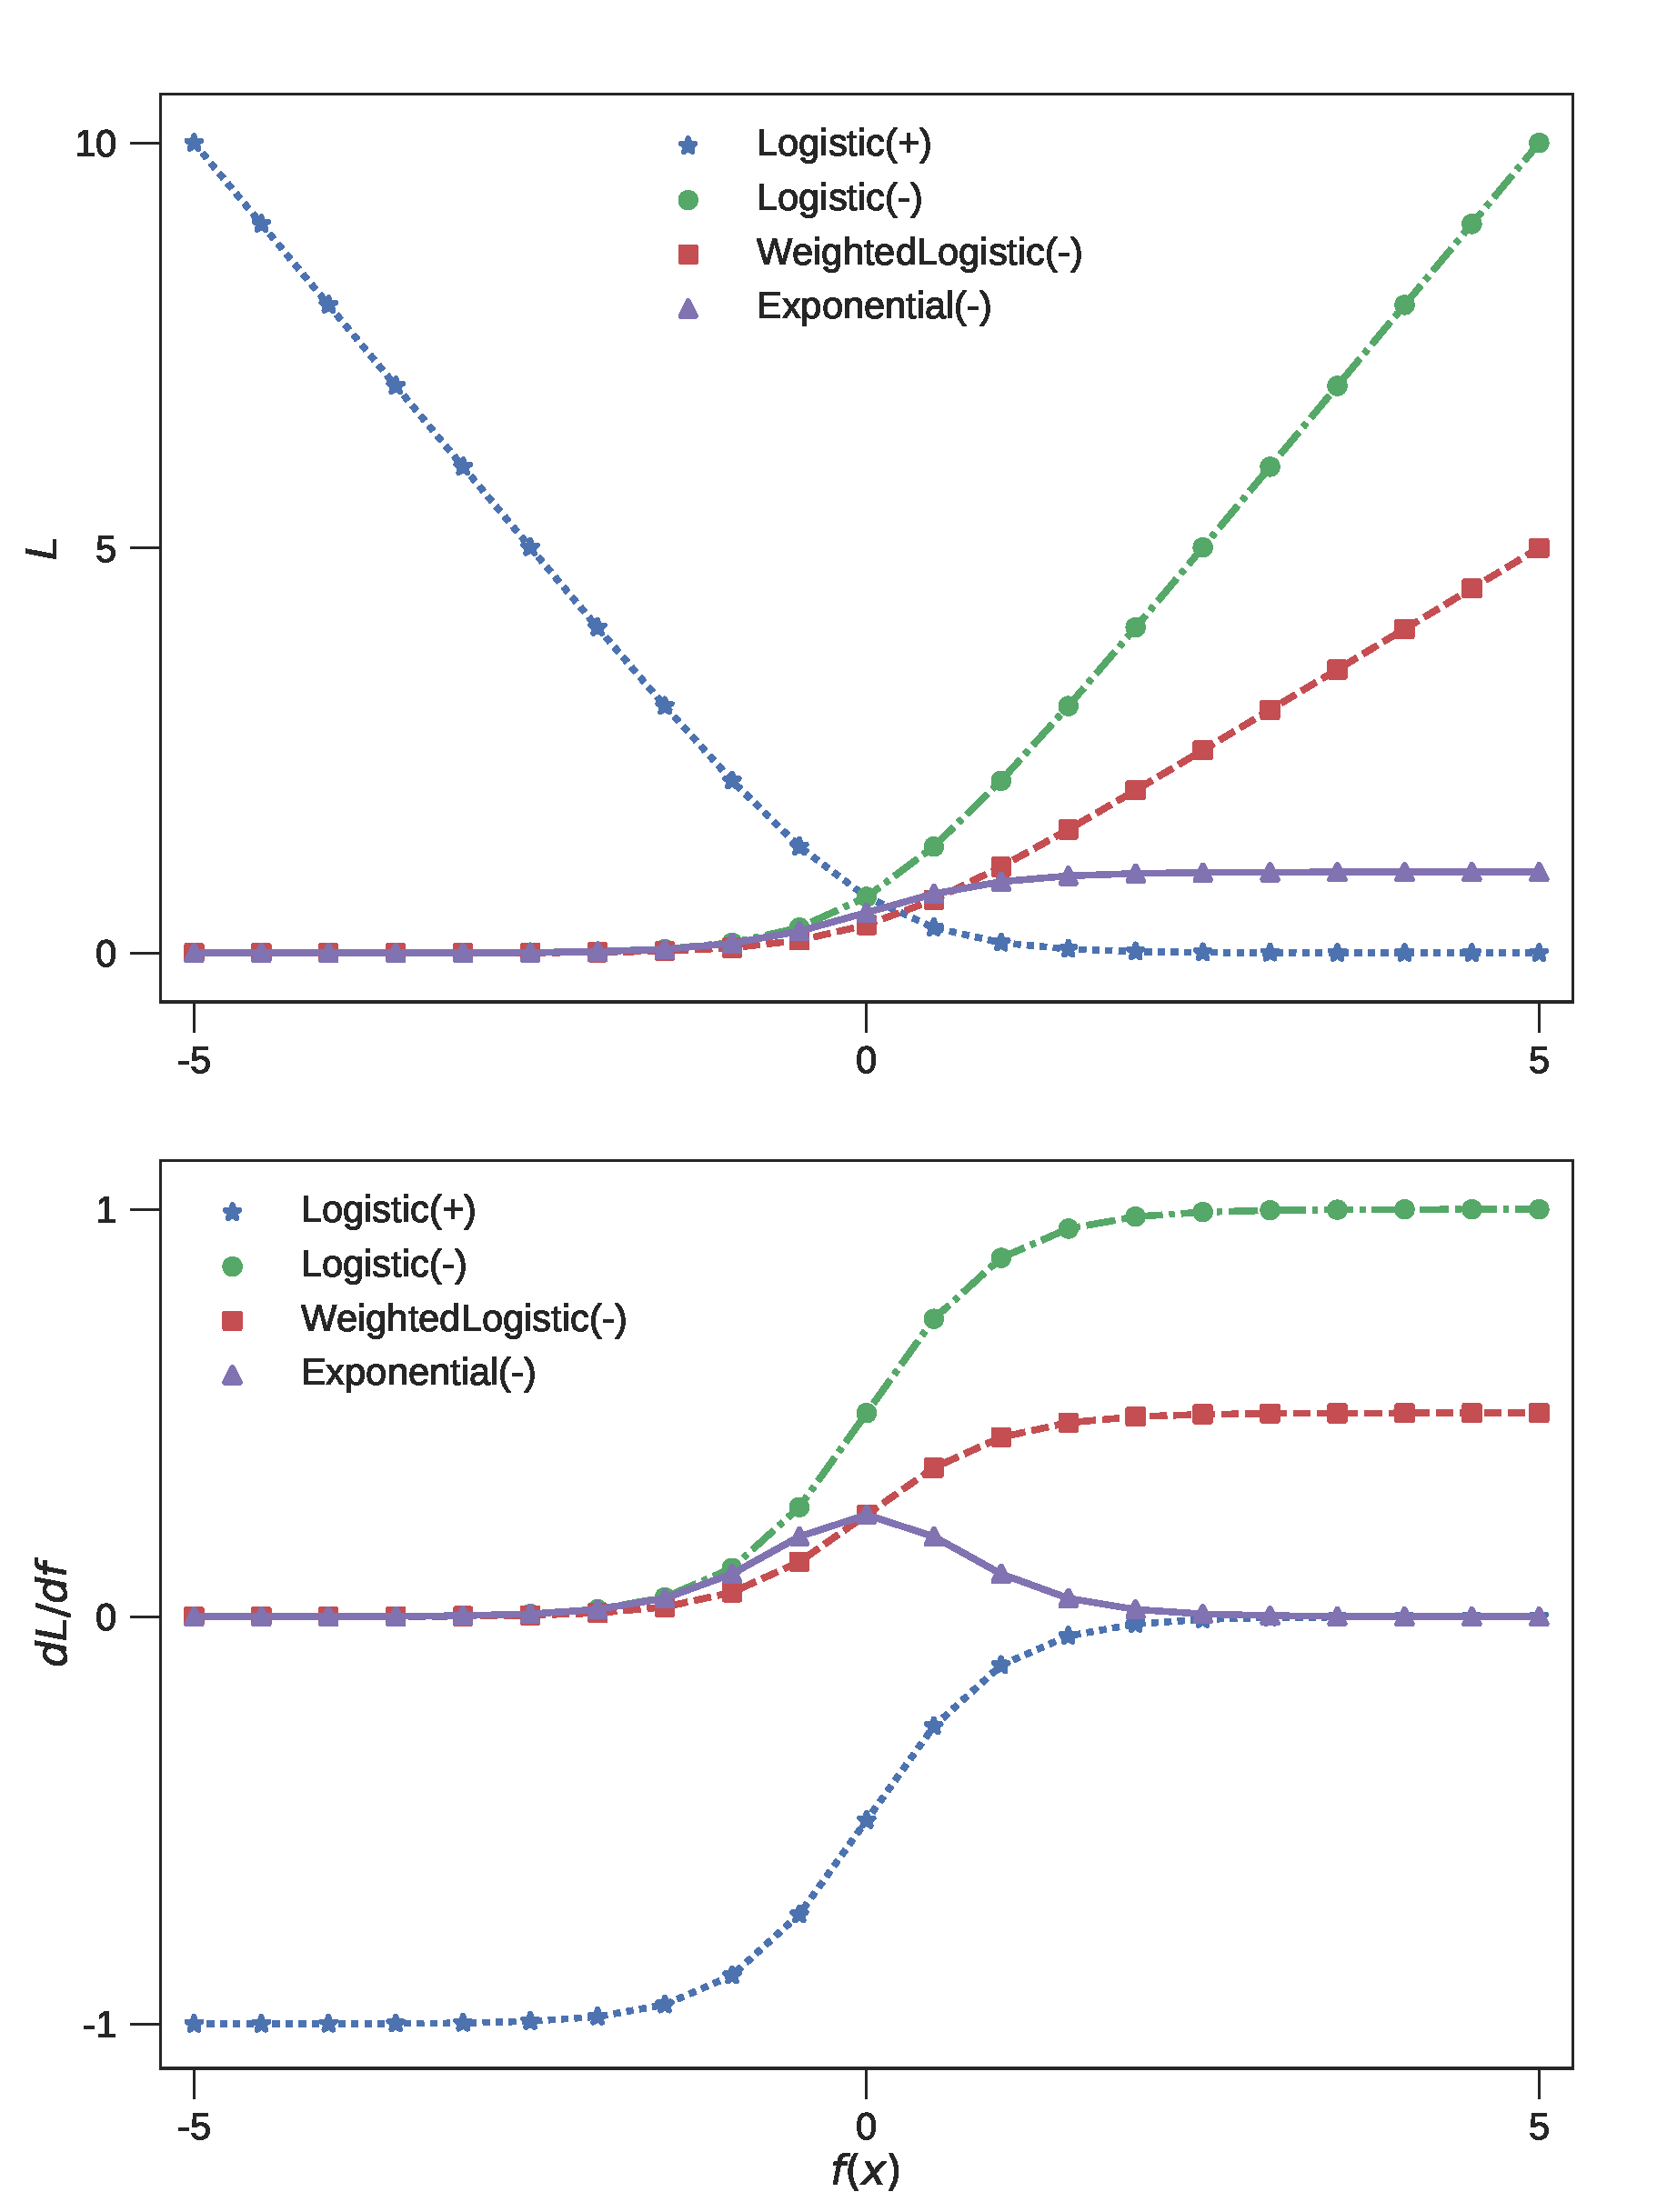
\includegraphics[width=1.05\linewidth]{img/losses}
\caption{
The differences in losses (top figure) and derivatives (bottom figure) with repect to the model output $f$ between the weighted logistic loss and the sigmoid loss for the negative class.
The \textbf{+} sign represents the loss of positive samples and the \textbf{-} sign stands for the loss of negative samples.
The sigmoid loss of negative examples reaches a plataeu and the derivative drops to zero in the very positive region.
The weighted logistic loss for negative is a linearly scaled logistic loss.
}
\label{fig:losses}
\end{figure}

%%%%%%%%%%%%%%%%%%%%%%%%%%%%%%%%%%%%%%%%%%%%%%%%%%%%%%%%%%%%%%%%%%%%%%
%%%%%%%% TEXT PU Learning setup
%%%%%%%%%%%%%%%%%%%%%%%%%%%%%%%%%%%%%%%%%%%%%%%%%%%%%%%%%%%%%%%%%%%%%%

\paragraph{PU Learning}

A training set for the positive and negative (PU) learning problems contains only a set of positive examples (P set) and a set of unlabeled samples (U set).
Unlabeled examples can be either positive or negative, meaning that there is no reliable negative examples available
One straightforward way to generate negative examples for training is to treat all the unlabeled examples as a set of negative examples with noises.
The problem then converts to learning with clean positive labels and noisy negative labels.
The goal of solving a PU learning problem is to learn a classifier that predicts as many positives as possible while keeping the false positive rate low, regardless the influence of false negative labels.
In other words, the purpose is to achieve high recall without sacrificing too much precision.


%%%%%%%%%%%%%%%%%%%%%%%%%%%%%%%%%%%%%%%%%%%%%%%%%%%%%%%%%%%%%%%%%%%%%%
%%%%%%%% TEXT Weighted loss for negatives
%%%%%%%%%%%%%%%%%%%%%%%%%%%%%%%%%%%%%%%%%%%%%%%%%%%%%%%%%%%%%%%%%%%%%%

\paragraph{Weighted logistic loss}

The mislabeled negative samples bias the classifier to have low recall.
It is possible to balance precision and recall by simply weighing the positive and negative examples differently, namely, let the positive and negative examples have different rates of contribution to the total loss.
Suppose a logistic loss is used, the corresponding weighted loss for a input-output pair $(x, y)$ for a classifier determined by parameters $\theta$ is:
\[
  l(x, y; \theta) =
    \begin{cases}
      - \alpha \log P(y=+1 \vert x; \theta), & y = +1 \\
      - \beta \log P(y=-1 \vert x; \theta), & y = -1
    \end{cases}
\]
where $\alpha$ and $\beta$ are weights for positive and negative class respectively, and $P(y\vert x; \theta)=\sigma(f(x; \theta))$ is the probablistic predictions by model $f(\cdot)$, activated by the sigmoid function $\sigma(\cdot)$.
This loss is referred to as the \textbf{weighted loss} in the rest of paper.
Empirically, the choice of $p$, $q$ can be made based on the highest precision and recall achieved on a validation set, or alternatively based on a class priors estimation\cite{du2014class}.
% Alternatively, one can also roughly assign $q=p(y=-1 \vert \tilde{y}=-1)$.
% This turns out to be part of the backward corrected loss proposed in  \cite{patrini2016making}:
% \begin{equation*}
%   \begin{aligned}
%     l_{\tilde{y_i}=-1} = - p(y_i=-1 \vert \tilde{y_i}=-1) \log p(y_i=-1 \vert x_i) \\ - p(y_i=+1 \vert \tilde{y_i}=-1) \log p(y_i=+1 \vert x_i)
%   \end{aligned}
% \end{equation*}
% % $$p( \tilde{y} \vert x, y) = \sum_{y}p(\tilde{y} \vert y)p(y \vert x)$$
% % $$p(y=+1 \vert \tilde{y}=+1) = 1 $$
% % $$p(y=-1 \vert \tilde{y}=+1) = 0 $$
% with $p(y_i=-1 \vert \tilde{y_i}=-1) = q$ and $p(y_i=+1 \vert \tilde{y_i}=-1) = 1-q$.



%%%%%%%% TEXT sigmoid Negative loss
\paragraph{Sigmoid Loss for the negative class}

As motivated in Section \ref{sec:related}, we used a class-dependent loss to down-weight the loss contribution of very positive predictions negative labels and still making full use of the clean positive labels.
The loss of positive examples is still a normal logistic loss and the loss of negative examples is replaced with a sigmoid loss \cite{tax2016class}:
\[
  l(x, y; \theta) =
    \begin{cases}
      - \log P(y=+1 \vert x; \theta), & y = +1 \\
      1 - P(y=-1 \vert x; \theta), & y = -1
    \end{cases}
\]
We called this class-dependent loss \textbf{sigmoid loss} in a sense it uses a sigmoid function as the loss of negative samples.
Using the logistic loss for the positive class and the sigmoid loss for the negative class is an interpretation of the prior knowledge that the positive labels are reliable whereas the negative labels are not.

Figure \ref{fig:losses} shows the differences in losses and derivatives with respect to model output between weighted logistic loss and sigmoid loss.
The main feature of sigmoid loss for negative examples is its small changes in the region of confident positive, compared to the weighted loss with $\alpha=1$ and $\beta=0.5$.
As a consequence, the corresponding derivative decreases to zero as the model prediction increases in the positive direction.


%%%%%%%% TEXT Bootstrapping
\paragraph{Hard bootstrapping loss for the negative class}
In addition to the proposed sigmoid loss, we also modify the hard bootstrapping loss by Reed et al. \cite{reed2014training} for PU learning to set a benchmark.
The modified class-dependent hard bootstrapping loss a pair of inputs and label $(x,y)$ is:
% $$l_- = - \beta \log p(y=-1 \vert x) - (1-\beta) \sum_{j\in \{-1, +1\}} p(y=j \vert x) \log p(y=j \vert x)$$
\begin{equation*}
\resizebox{\columnwidth}{!}{$
  l(x, y; \theta) =
    \begin{cases}
      - \log P(y=+1 \vert x; \theta), & y = +1 \\
      - \beta \log P(y=-1 \vert x;\theta) - (1-\beta) \log P(y=\hat{y} \vert x;\theta), & y = -1
    \end{cases}
$}
\end{equation*}
where $\hat{y} = \argmax_{j\in\{-1,+1\}}{P(y=j \vert x)}$ is the class with the highest predicted probability and $0<\beta<1$.
The first term of the objective is a weighted logistic loss and the second term can be considered as a regularization term to encourage consistent predictions.
This loss is referred as \textbf{bootstrapping loss} for the rest of this paper.
% \begin{equation*}
%   \begin{aligned}
%     H = - \sum_{j\in\{-1,+1\}} p(y_i=j \vert x_i) \log p(y_i=j \vert x_i) \\
%     \sim - \sum_{j\in\{-1,+1\}} \delta(y_i - \hat{y_i}) \log p(y_i=j \vert x_i)
%   \end{aligned}
% \end{equation*}
% which intuitively encourages the model to make confident predictions \cite{grandvalet2005semi}.

%%%%%%%% TEXT Segmentation
\paragraph{Extending PU learning from classification to segmentation}
In Section \ref{introduction}, we argue that learning with unlabeled foreground pixels is similar to a PU learning setup.
Howvever, there is still differences between learning with unlabeled foreground pixels and learning with positive and unlabeled examples.

The first difference is that each example in the normal PU learning setup is independent of each other, whereas pixels in images are not.
Assuming the probability of mislabeling foreground pixel as the background is independent of its neighbor pixels, the classification losses can be applied to segmentation problems by performing per-pixel classification problems.

Another difference between incomplete segmentation and a normal positive and unlabeled learning problem is that pixels for objects of various categories can be unlabeled.
Supposing there are $K$ categories of interest, varying from class $1$ to class $K$, the class $0$ is for unlabeled data which may or may not belong to the $K$ defined categories.
The sigmoid loss can be extended train deep learning models with unlabeled examples from various categories:

\[
  l(x, y; \theta) =
    \begin{cases}
      - \alpha_1 \log P(y=1 \vert x; \theta), & y = 1 \\
                                              & \vdots \\
      - \alpha_K \log P(y=K \vert x; \theta), & y = K \\
      \beta (1 - P(y=0 \vert x; \theta)), & y = 0
    \end{cases}
\]
where $\alpha_1, \dots, \alpha_K, \beta$ are weighting factors, and $P(y \vert x; \theta)$ is the predictied probability for class $y$, i.e., model output activated by the softmax function.
This loss is referred to as the \textbf{softmax loss} because it uses a softmax activation for the model output.

% Similar modifications can be made to the cross-entropy loss, namely, keeping the losses for classes $1$ to $K$ unchanged and applying the loss for negative class to the loss for class 0, supposing there are $K$ positive classes and one negative class.
% Alternatively, one can apply a one-vs-all strategy, with which the normal logistic loss is used for positive classes while the weighted, sigmoid and bootstrapping loss can be used for the negative class.

%%%%%%%% TEXT Expontial loss FADE IN
\paragraph{Implementation details}
We introduced the sigmoid loss only after training with a class-weighted cross entropy loss for a few epochs.
The sigmoid loss of negative examples saturates for very positive outputs, meaning that the confident, positive prediction has little contribution to the weights update.
The wrong confident predictions can introduce problems at the beginning of the training procedure when the confident predictions are likely to be made at random.
Otimization would reach the plateau when the model made all positive predictions with high confidence.
Besides, we also introduce the modified hard bootstrapping loss only after a few epochs trained with class-weighted loss because it also relies on a nonrandom model for sufficiently reliable prediction $\hat{y}$.


%%%%%%%% TEXT Imbalanced

Another problem encountered in the PU learning setup is the class imbalance introduced by negatively labeled positive samples.
A balanced dataset can become imbalanced in the presence of false negative labels, especially if only a small portion of positive samples are correctly labeled.
We reweighed positive and negative samples based on their occurrences of the observed labels to alleviate the influence of imbalance for training.
Note that the class-weighted logistic loss reweighed the classes in addition to this frequency balancing class weight.


\section{Results}
\label{sec:results}
\subsection{Impact of label noise on feature transferability}


%%%%%%%% FIGURE Number of training categories
\begin{figure}[t]
\centering
   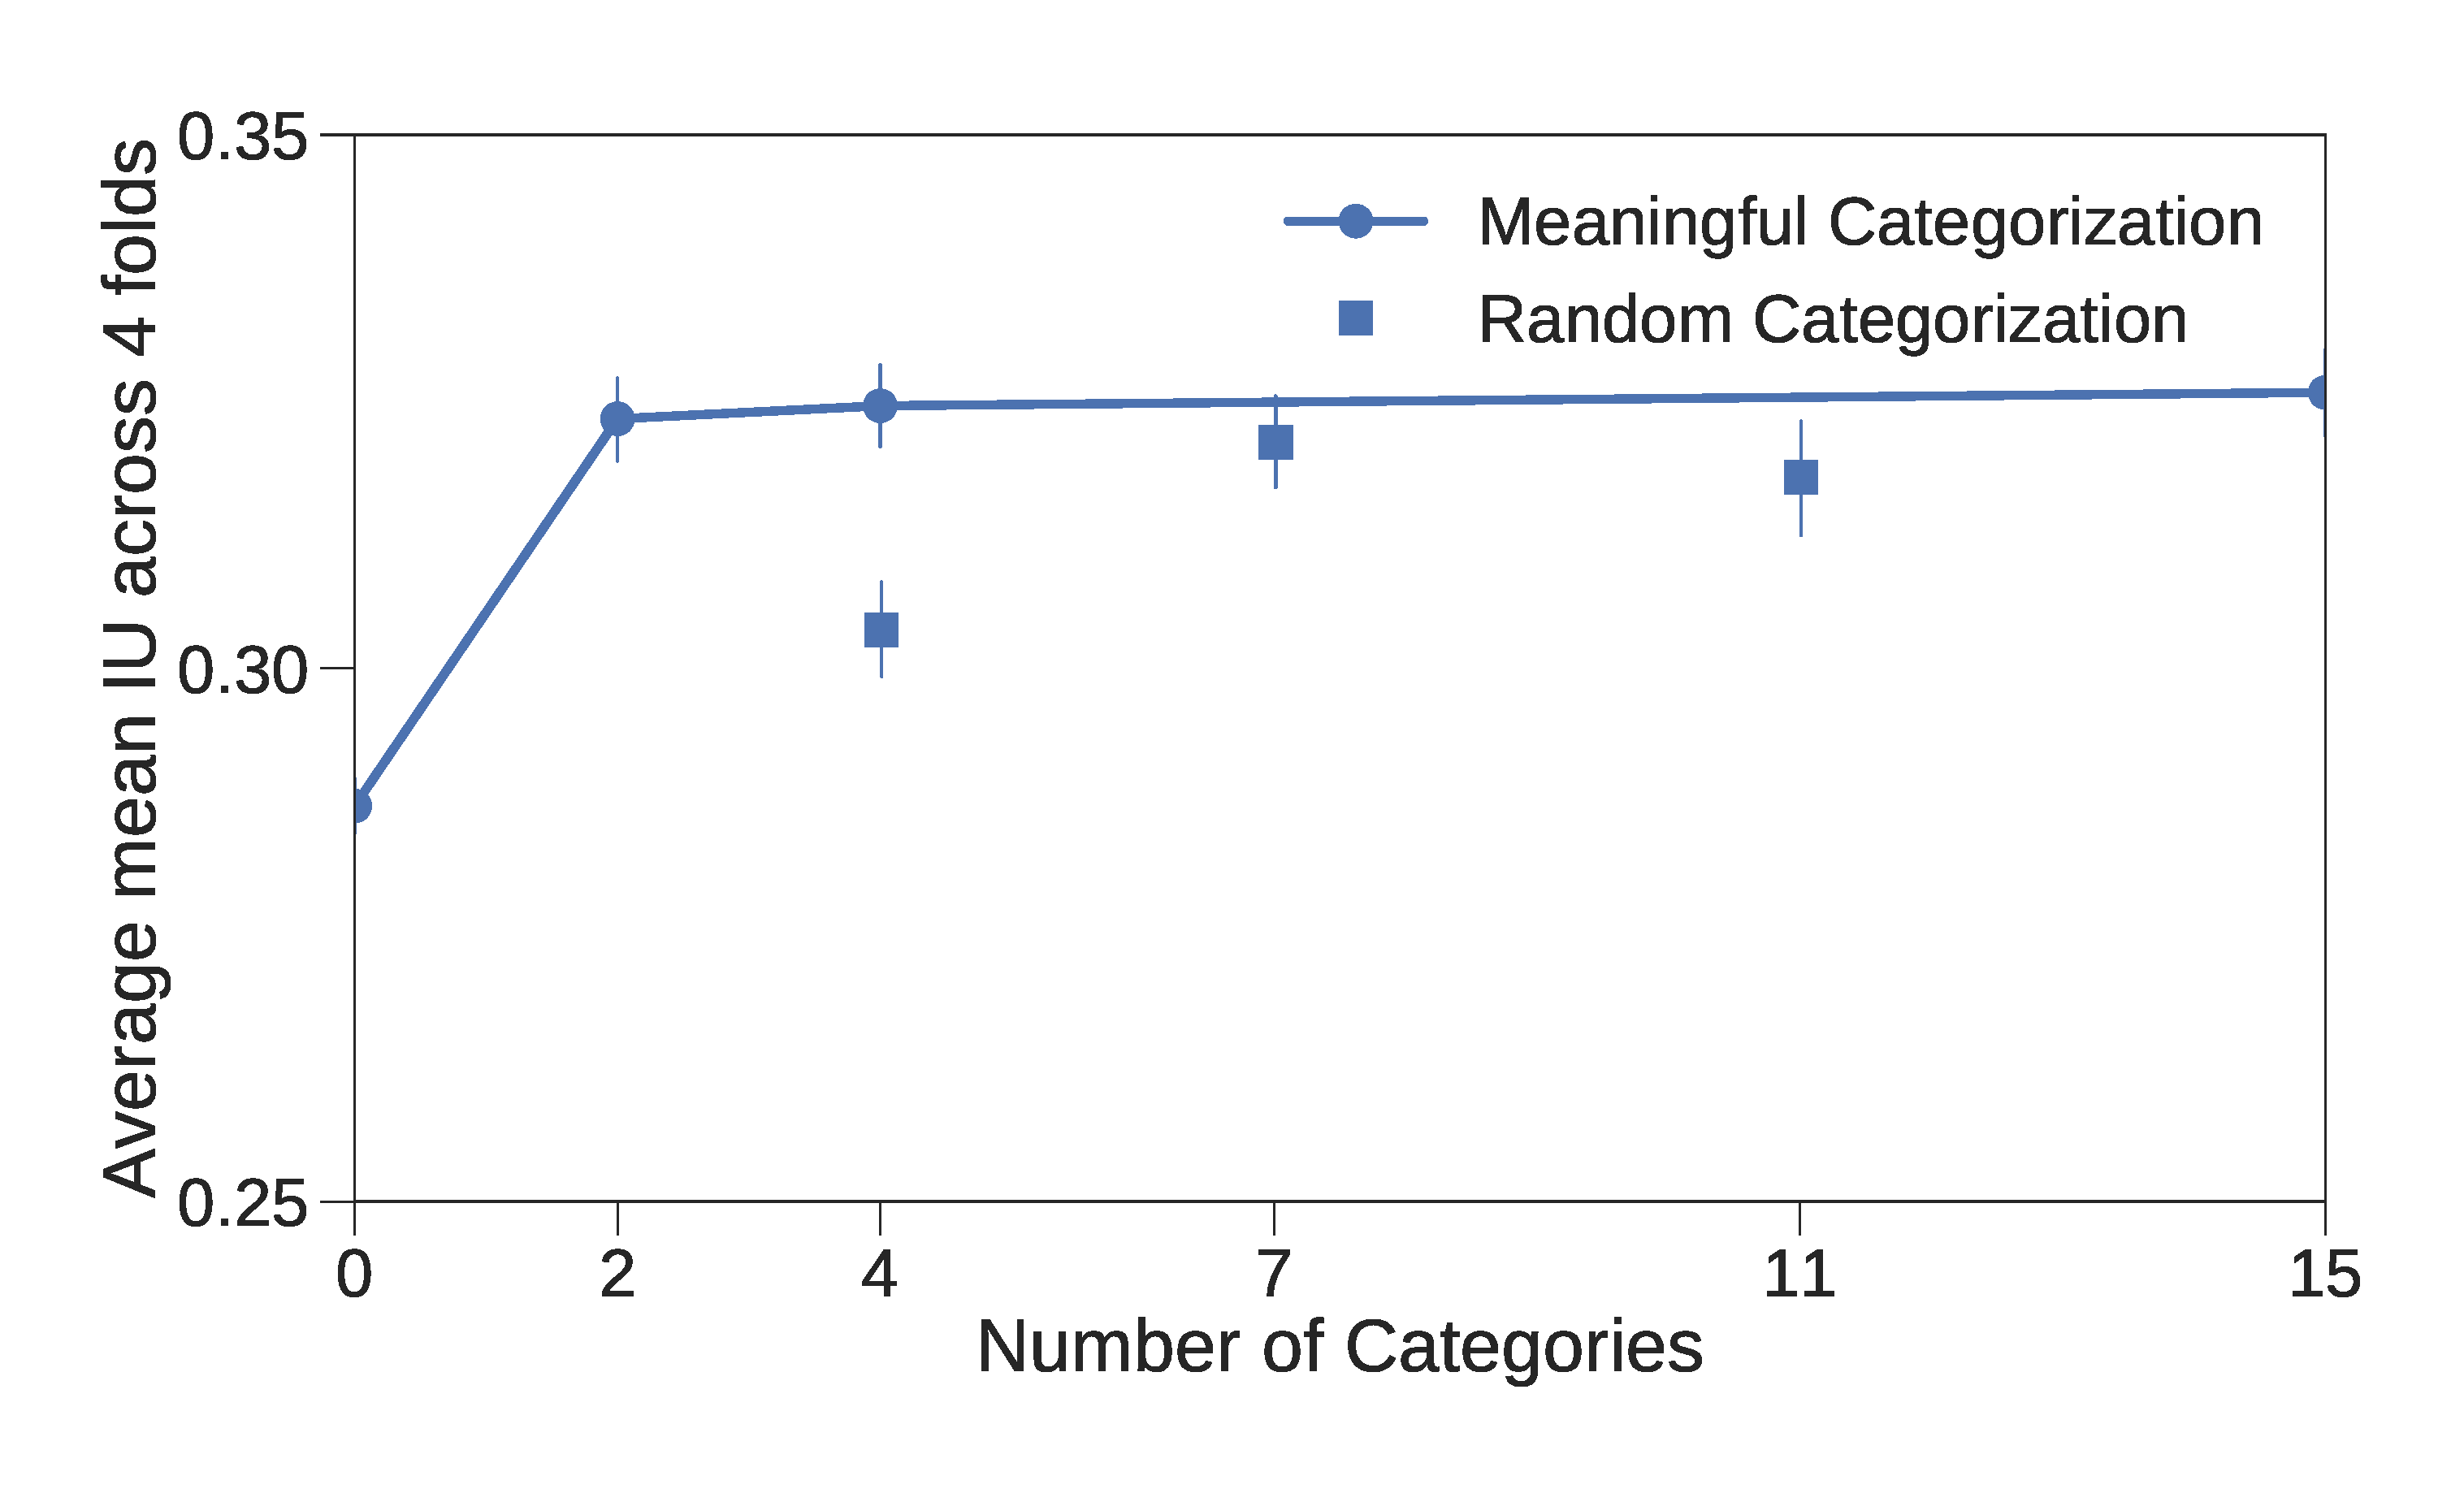
\includegraphics[width=1.\linewidth]{img/num_classes.eps}
\caption{
The influence of number of categories in the pre-training dataset on performance of fine-tuned models.
Varying the number of categories while pre-training the representation and the pre-trained weights were fine-tuned to segment 5 categories from the PASCAL VOC2011 dataset
}
\label{fig:categories}
\end{figure}

% %%%%%%%% FIGURE First-layer feature visualization
% \begin{figure}[t]
% \centering
% \fbox{\rule{0pt}{2in} \rule{0.9\linewidth}{0pt}}
%   %  \includegraphics[width=0.95\linewidth]{img/}
% \caption{Visualization of first-layer features from different pre-trained models.}
% \label{fig:features}
% \end{figure}


\section{Conclusion}
\label{sec:conclusion}

We studied how to pre-train transferable convolutional weights in the presence of inexhaustive segmentation, misclassification and false segmentation.
We discovered that including false segmentations of meaningful objects for pre-training had little impact on the fine-tuning performance of transferred weights
By contrast, misclassification noises can have negative impacts on feature transferability, but binarizing classes to foreground and background can produce accurate but not necessarily precise labels to train better transferable features.
We presented that for a small pre-training set, binarizing classes can recover the negative influence of misclassification of object segments on the fine-tuning performance of the transferred models.
Inexhaustive segmentation can also negatively affect feature transferability of the pre-trained model.
The decrease of the fine-tuning performance due to the unsegmented objects in the pre-training set can be compensated by modifying the loss function for deep learning models.
We then proposed a class-dependent loss to not over-punish the confident positive predictions for examples with negative labels.
The proposed sigmoidal negative loss was demonstrated to improve both the pre-training and fine-tuning performance of models pre-trained in the presence of inexhaustive segmentations.



{\small
\bibliographystyle{plain}
\bibliography{references}
}

\end{document}
